\documentclass[10pt]{amsart}
\usepackage{amsmath}
\usepackage{amsthm}
\usepackage{tikz}
\usetikzlibrary{shapes.geometric, arrows}


\usepackage{minted}


\newcommand{\R}{\mathbb{R}}
\newcommand{\C}{\mathcal{C}}


\newtheorem{theorem}{Theorem}[section]
\newtheorem{proposition}[theorem]{Proposition}
\newtheorem{lemma}[theorem]{Lemma}
\newtheorem{corollary}[theorem]{Corollary}


\theoremstyle{definition}
\newtheorem{definition}[theorem]{Definition}
\newtheorem{example}[theorem]{Example}


\begin{document}
\title{Recurrent Neural Networks}
\author{Jean-Martin Albert}
\date{\today}
\maketitle





%\def\layersep{2.5cm}


% \newcommand{\nodedef}{\tikzstyle{arrow} = [thick,->,>=stealth]
%     \node (input) [] at (0cm,1cm) {};
%     \node (output) [] at (0cm,-1cm) {};
%     \node (s-input) [] at (-2cm,0cm) {};
%     \node (s-output) [] at (2cm,0cm) {};
%     \path[yshift=0.5cm]
%         node[startstop] (N) at (0cm,-.5cm) {};
%
%     \draw [arrow] (input) -- (N);
%     \draw [arrow] (s-input) -- (N);
%     \draw [arrow] (N) -- (output);
%     \draw [arrow] (N) -- (s-output);}
%
%
% \newcommand{\nodedefinner}{\tikzstyle{arrow} = [thick,->,>=stealth]
%     \node (input) [] at (0cm,1cm) {};
%     \node (output) [] at (0cm,-1cm) {};
%     \node (s-input) [] at (-2cm,0cm) {};
%     \node (s-output) [] at (2cm,0cm) {};
%     \path[yshift=0.5cm]
%         node[startstop] (N) at (0cm,-.5cm) {};
%
%     %\draw [arrow] (input) -- (N);
%     %\draw [arrow] (s-input) -- (N);
%     \draw [arrow] (N) -- (output);
%     \draw [arrow] (N) -- (s-output);}


% \begin{tikzpicture}[shorten >=1pt,->,draw=black!50, node distance=1cm]
%     \tikzstyle{arrow} = [thick,->,>=stealth]
%     \tikzstyle{startstop} = [rectangle, minimum width=2cm, minimum height=.75cm, text centered, draw=black, fill=black!20]
%     \node (input) [] at (0cm,1cm) {};
%     \node (output) [] at (0cm,-1cm) {};
%     \node (s-input) [] at (-2cm,0cm) {};
%     \node (s-output) [] at (2cm,0cm) {};
%     \path[] node[startstop] (N) at (0cm,0cm) {};
%     \draw [arrow] (input) -- (N);
%     \draw [arrow] (s-input) -- (N);
%     \draw [arrow] (N) -- (output);
%     \draw [arrow] (N) -- (s-output);
% \end{tikzpicture}
%
%








 \section{Introduction}

 Let $U=\R^n$ and $V=\R^m$ be vector spaces, and consider a function $f:U\to W$.
 In theory, $f$ here can be any set theoretic function, but for our purpose, we
 will assume that $f$ is at the very least square integrable. In general, we
 consider a class $\C$ of functions $U\to V$, and try to find an element $g\in\C$
 which is as close as possible to $f$.  In order to do so, we need a notion of distance
 between functions.  There are many possible choices, but some of the most popular are
 the $L^p$ norms and the $L^\infty$ norm.

 While the class $\C$ van be virtually any class of functions, we usually choose a class
 that is somewhat definable, in the sense that there is a (differentiable) function $F:U\times\R^k\to V$
 such that $\C=\{F(x, w): w\in \R^k\}$.  Such classes of functions have the advantage of
 being equicontinuous.


 \begin{example}
 Let $f(x)=x(x-1)(x+1)$.  As an example, we will try to fit a linear function
 $\ell(x)=ux+v$ to $f$.  The class $\C$ is defined by $\C=\{ux+v:u,v\in R\}$.
 For an element $g(x, u, v)\in\C$, we have $$f(x)-g(x,u,v) = x^3-x - ux+v$$
 From this we get
 \begin{eqnarray*}
   (f(x)-g(x,u,v))^2 &=& (x^3 - (1-u)x + v)^2 \\
   {} &=& x^6 - 2(1-u)x^4 + 2vx^3 + (1-u)^2x^2 - \\
   {} & & 2(1-u)vx + v^2
 \end{eqnarray*}
 If we compute $\int_{-1}^1 (f(x)-g(x,u,v))^2$, we get

 \begin{eqnarray*}
   \int_{-1}^1(f(x)-g(x; u,v))^2 &=& \int_{-1}^1(x^3 - (1-u)x + v)^2 \\
   {} &=& \int_{-1}^1x^6 - 2(1-u)x^4 + 2vx^3 + (1-u)^2x^2 - 2(1-u)vx + v^2\\
   {} &=& \frac{x^7}{7}-2v\frac{x^4}{4} + (1-u)^2\frac{x^3}{3} - 2(1-u)v\frac{x^2}{2}+v^2x\\
   {} &=& \frac{1}{7}-2v\frac{1}{4} + (1-u)^2\frac{1}{3} - 2(1-u)v\frac{1}{2}+v^2\\
   {} & & +\frac{1}{7}-2v\frac{1}{4} + (1-u)^2\frac{-1}{3} - 2(1-u)v\frac{1}{2}-v^2\\
   {} &=& \frac{2}{7} - (2-u)v+v^2 = \ell(u,v)
 \end{eqnarray*}
 and note that the last line above is a function of $u$ and $v$ alone, and we have to minimize it.
 \end{example}




\section{Back Propagation}

In general, in order to minimize a function $f(w)$ of one variable, we make use of the fact that
the extreme values of $f$ all have $f'(x)=0$.  If $f$ is a function of two or more variables, then
if $x$ is such that $f(x)$ is a local max, or minimum, then all partial derivatives
$\frac{\partial f}{\partial w_i}(x)=0$.  If $f:\R^n\to\R$ is a function, then the
{\em gradient} of $f$ is the vector
$\nabla f(x) = \left(\frac{\partial f}{\partial w_1}(x),...,\frac{\partial f}{\partial w_n}(x)\right)$.
One interesting property of $\nabla f(x)$ is that, as a vector, it ``points'' in the direction in which
$f$ decreases the most.  That is to say, there is a good chance that $f(x-\alpha\nabla f(x))\leq f(x)$.
The chance is better the smaller $\alpha$ is.  We see that if we iterate that process, we get a
sequence $x_1,...,x_n,...$ such that $f(x_{i+1})\leq f(x_i)$ for every $i$.  Since $m\leq f(x_i)\leq f(x_0)$
for every $i$, we get a bounded decreasing sequence of real number, which converges.

Caveat: this ideal situation doesn't allways happen.

This iterative process is {\em (Stocastic) gradient descent}.

Suppose $f$ is a complsition of two functions, and that we can write $f(x,w)= g(h(x, w_1), w_2)$.
Then we can write $\nabla_w f(x, w)=\nabla g(h(x, w_1), w_2)\cdot \nabla h(x, w_1)$. Each level
of composition corresponds to a layer of neural network.  The chain rule transforms function composition
into a product. If a network becomes deep, then the derivative of the loss function becomes a long
product.  When gradients become small in norm (like they do when we approach a min), then the gradient
becomes very close to $0$, and the update rule for gradient descent stops changing the weights.

This is the vanishing gradient problem for very deep networks, and makes convergence slow.

\section{Dealing with sequences}

Let $A$ be a finite set. We define the set $A^*$ of all finite sequences of elements of $A$ to be the smallest set $X$ with the property that the empty sequence $\epsilon$ is in $X$, and whenever $w\in X$ and $a\in A$, the sequence $aw\in X$. If $A$ and $B$ are two finite sets, and $f:A\to B$ is any function, then we can extend $f$ extends uniquely to a function $f^*:A^*\to B^*$, which is defined by $f(a_1a_2,...,a_n)=f(a_1)f(a_2)\cdots f(a_n)$. This $f^*$ is the only function extending $f$ which satisfies $f(vw)=f(v)f(w)$.

Let $S$ be another finite set with a distinguished element $\perp\in S$, and let $f:A\times S\to B\times S$ be a function. We can use $f$ to define a function $f^*:A^*\to B^*$ in several ways. Consider an auxiliary function $f^*:A^*\to B^*\times S$ by defining First we define $f^*(\epsilon)=(\epsilon, \perp)$. If $a\in A$ then $f^*(a)=f(a, \perp)$. If $v=aw$, then by induction we can compute $f^*(w)=(u, s)$. Write $f(a, s)=(b, s')$, and define $f^*(aw)=(bu, s')$.  We can produce a function $f^*:A^*\to B^*$ by taking $f^*(w)=\pi_2 g(w)$.

We can use $f$ to define a function $f^*:A^*\to B$. Consider an auxiliary function $f^*:A^*\to B\times S$ by defining First we define $f^*(\epsilon)=(b_0, \perp)$. If $a\in A$ then $f^*(a)=f(a, \perp)$. If $v=aw$, then by induction we can compute $f^*(w)=(u, s)$. Write $f(a, s)=(b, s')$, and define $f^*(aw)=(b, s')$.  We can produce a function $f^*:A^*\to B$ by taking $f^*(w)=\pi_2 g(w)$.

Let $S$ be another finite set with a distinguished element $\perp\in S$, and let $f:A\times S\to B\times S$ be a function. We can use $f$ to define a function $f^*:A\to B^N$ for every $N$ in several ways. Consider an auxiliary function $f^*:A\to B^N\times S$ by defining. If $a\in A$ then $f^*(a)_1=f(a, \perp)$. Suppose $f^*(a)_n=(w, s)$, and  $f(a, s) = (b, s')$, then $f^*(a)_{n+1}=(bw, s')$.  This is an example of a one-to-many function. If $A$ has a distinguished element $a_0$, then we can define $f^*(a)_1=f(a, \perp)$, and $f^*(a)_n=(w, s)$, and  $f(a_0, s) = (b, s')$, then $f^*(a)_{n+1}=(bw, s')$.  This is an example of a one-to-many function.  Note that this is a special case of the many to many function, where $f^*(a)$ is just defined as $f^*(aaa\cdots a)$, or $f^*(aa_0\cdots a_0)$.


%If $v=aw$, then by induction we can compute $f^*(w)=(u, s)$. Write $f(a, s)=(b, s')$, and define $f^*(aw)=(bu, %s')$.  We can produce a function $f^*:A^*\to B^*$ by taking $f^*(w)=\pi_2 g(w)$.
%  We can then define $f^*(v)=f^*(aw)=f(a, s) = (w', s')$, or mode formally, $f^*(aw)=f(a, \pi_2f^*(w)$
%
%$f^*(v)=f^*()
%
%There is more than one way to extend a recurrent function to a set of sequences




\section{The base of recurrent networks}

Consider a function $f:U\times S\to V\times S$, where $U$, $V$ and $S$ are finite dimensional vector spaces.
Note that every vector space has a a distinguished element $0$, the zero-vector.  Let $u_1,...,u_n$ be a finite
sequence of vectors in $U$.  We construct a sequence of vectors in $V$ as follows. Write $f(u_1, 0)=(v_1, s_1)$,
and for every $i$, if $f(u_{i}, s_{i-1})=(v_i, s_i)$. Note that this is a state machine, close to a
deterministic finite automaton, except that here the state space $S$ is infinite.

The set $\{0,1\}^*$ of all finite sequences of $0$'s and $1$'s is countable, and $S$, being a real vector space,
is uncountable.  Therefore, we can encode every element $w\in\{0,1\}^*$ as a vector in $S$.  Informally,
$S$ is enough to encode any finite state space, and every possible value for the content of the tape of a
Turing machine. We get:

\begin{theorem}
Recurrent neural networks are Turing-complete.
\end{theorem}

which explains why recurrent neural networks seem to be able to produce results that other networks can't.
Training a recurrent network is the same as producing a Turing machine.

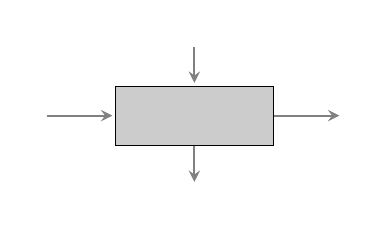
\begin{tikzpicture}[shorten >=1pt,->,draw=black!50, node distance=1cm]
    \tikzstyle{arrow} = [thick,->,>=stealth]
    \tikzstyle{startstop} = [rectangle, minimum width=2cm, minimum height=.75cm, text centered, draw=black, fill=black!20]
    \node (input) [] at (0cm,1cm) {};
    \node (output) [] at (0cm,-1cm) {};
    \node (s-input) [] at (-2cm,0cm) {};
    \node (s-output) [] at (2cm,0cm) {};
    \path[] node[startstop] (N) at (0cm,0cm) {};
    \draw [arrow] (input) -- (N);
    \draw [arrow] (s-input) -- (N);
    \draw [arrow] (N) -- (output);
    \draw [arrow] (N) -- (s-output);
\end{tikzpicture}

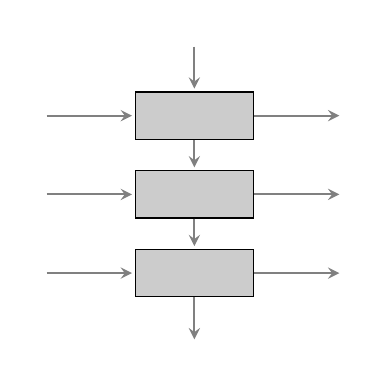
\begin{tikzpicture}[shorten >=1pt,->,draw=black!50, node distance=1cm]
    \tikzstyle{arrow} = [thick,->,>=stealth]
    \tikzstyle{startstop} = [rectangle, minimum width=1.5cm, minimum height=.6cm, text centered, draw=black, fill=black!20]
    \node (input) [] at (0cm,1cm) {};
    \node (output) [] at (0cm,-3cm) {};
    \node (s-input-A) [] at (-2cm,0cm) {};
    \node (s-output-A) [] at (2cm,0cm) {};
    \node (s-input-B) [] at (-2cm,-1cm) {};
    \node (s-output-B) [] at (2cm,-1cm) {};
    \node (s-input-C) [] at (-2cm,-2cm) {};
    \node (s-output-C) [] at (2cm,-2cm) {};
    \path[] node[startstop] (A) at (0cm,0cm) {};
    \path[] node[startstop] (B) at (0cm,-1cm) {};
    \path[] node[startstop] (C) at (0cm,-2cm) {};
    \draw [arrow] (input) -- (A);
    \draw [arrow] (s-input-A) -- (A);
    \draw [arrow] (s-input-B) -- (B);
    \draw [arrow] (s-input-C) -- (C);
    \draw [arrow] (A) -- (s-output-A);
    \draw [arrow] (B) -- (s-output-B);
    \draw [arrow] (C) -- (s-output-C);
    \draw [arrow] (A) -- (B);
    \draw [arrow] (B) -- (C);
    \draw [arrow] (C) -- (output);
\end{tikzpicture}




\section{Backward Propagation Through Time}

How do we train recurrent neural networks? we can use back propagation, just like a regular neural network. Heuristically, we unroll the recurrent network ``infinitely'' many times, until it looks like an ordinary very deep neural network.  In practice, since computers only have a finite amount of resources, we only unroll the network a large but finite number of times, and treat it like an ordinary neural network.

\begin{tikzpicture}[shorten >=1pt,->,draw=black!50, node distance=1cm]
    \tikzstyle{arrow} = [thick,->,>=stealth]
    \tikzstyle{startstop} = [rectangle, minimum width=1.5cm, minimum height=.6cm, text centered, draw=black, fill=black!20]
    \node (input) [] at (0cm,1cm) {};
    \node (output) [] at (0cm,-1cm) {};
    \node (s-input-A) [] at (-2cm,0cm) {};
    \node (s-output-A) [] at (10cm,0cm) {};
    %\node (s-input-B) [] at (-2cm,-1cm) {};
    %\node (s-output-B) [] at (10cm,-1cm) {};
    %\node (s-input-C) [] at (-2cm,-2cm) {};
    %\node (s-output-C) [] at (10cm,-2cm) {};
    \path[] node[startstop] (A-0) at (0cm,0cm) {};
    %\path[] node[startstop] (B-0) at (0cm,-1cm) {};
    %\path[] node[startstop] (C-0) at (0cm,-2cm) {};
    \draw [arrow] (input) -- (A);
    \draw [arrow] (s-input-A) -- (A-0);
    %\draw [arrow] (s-input-B) -- (B-0);
    %\draw [arrow] (s-input-C) -- (C-0);
    %\draw [arrow] (A) -- (B);
    %\draw [arrow] (B) -- (C);
    \draw [arrow] (A) -- (output);

     \foreach \i/\j in {1/0,2/1,3/2,4/3}
     {
       \node (input-\i) [] at (2*\i cm,1cm) {};
       \node (output-\i) [] at (2*\i cm,-1cm) {};
       \path[] node[startstop] (A-\i) at (2*\i cm,0cm) {};
    %   \path[] node[startstop] (B-\i) at (2*\i cm,-1cm) {};
  %     \path[] node[startstop] (C-\i) at (2*\i cm,-2cm) {};
  %     \draw [arrow] (A-\i) -- (B-\i);
%       \draw [arrow] (B-\i) -- (C-\i);
       \draw [arrow] (input-\i) -- (A-\i);
       \draw [arrow] (A-\j) -- (A-\i);
%       \draw [arrow] (B-\j) -- (B-\i);
%       \draw [arrow] (C-\j) -- (C-\i);
       \draw [arrow] (A-\i) -- (output-\i);
     }
     \draw [arrow] (A-4) -- (s-output-A);
     %\draw [arrow] (B-4) -- (s-output-B);
     %\draw [arrow] (C-4) -- (s-output-C);

\end{tikzpicture}



\section{Types of Recurrent Cells}

There are three main types of recurrent cells which are used to build recurrent neural networks.  Let us describe them, and give some of their basic properties, along with a na\"ive implementation in tensorflow.

\subsection{Basic Recurrent Cell} We begin with the most basic of recurrent cell. Abstractly, a function $f:U\times S\to V\times S$ can be defined using two functions $u:\R^n\times \R^\ell\to \R^n$ and $v:\R^n\times\R^\ell \to \R^\ell$. We se ethe former function as providing the output, and the latter function as a state updating function.  The most common definition for $u$ and $v$ for basic recurrent cells is as follows: $u(x, s) = f(A_ux+B_us)$, where $A$ nad $B$ are matrices, and $f$ is a non-linear function, and $v(x, s) = \tanh(A_vx+B_vs)$. Te parameters in this definition are $A_u$, $B_u$, $A_v$ and $B_v$. In tehsorflow, the code looks like:

\begin{minted}{python}
def basic_rnn_cell(input_tensor, state_tensor):
  A_u = tf.Variable(shape=[N, L])
  B_u = tf.Variable(shape=[L, L])
  A_v = tf.Variable(shape=[N, L])
  B_v = tf.Variable(shape=[L, L])
  output_tensor = tf.relu(tf.matmul(input_tensor, A_u) +
                            tf.matmul(state_tensor, B_u))
  new_state_tensor = tf.tanh(tf.matmul(input_tensor, A_v) + \
                                  tf.matmul(state_tensor, B_v))
  return output_tensor, new_state_tensor
\end{minted}


\subsection{Long Short-term Memory Cell} There are a few problems with the architecture described above.  First, it suffers greatly from the vanishing gradient problem, since there is no way to prevent gradients from becoming very small.  Secondly, simple recurrent networks have a hard time remembering facts about the input sequence.  To remedy this situation, long short-term memory cells were introduced.  The overall structure of an LSTM cell is almost the same as the basic RNN cell. This time we take the previous output into account, which gives the structure as $f:\R^n\times \R^m\times \R^{\ell}\to \R^m\times \R^{\ell}$ which can be divided as two function $u:\R^{n}\times\R^m\times \R^{\ell}\to \R^m$ and $v:\R^n\times \R^m\times\R^{\ell}\to \R^{\ell}$. To define the functione $u$ and $v$, we use auxiliary functions $F$, $I$, and $O$ defined as follows
\begin{eqnarray*}
  F(x, y) &=& \sigma(A_Fx + B_Fy + b_F)\\
  I(x, y) &=& \sigma(A_Ix + B_Iy + b_I)\\
  O(x, y) &=& \sigma(A_Ox + B_Oy + b_O)\\
  S(x, y) &=& \sigma(A_Ox + B_Oy + b_O)\\
\end{eqnarray*}
The state update is given by $v(x, y, s) = F(x, y)\circ s + I(x, y)\circ \sigma_v(A_vx + B_vy + b_v)$, where $\circ$ denotes pointwise multiplication of vectors, and finally, the output can be defined as $u(x, y, s)=O(x, y)\circ \sigma_u(v(x, y, s))$.

\begin{minted}{python}
def lstm_gate(input_tensor, previous_output, port_op):
  A = tf.Variable(shape=[N, L])
  B = tf.Variable(shape=[L, L])
  b = tf.Variable(shape=[L, L])
  x = tf.matmul(input_tensor, A)+ tf.matmul(previous_output, B) + b
  return post_op(x)

def lstm_cell(input_tensor, output, state):
  F = lstm_gate(input_tensor, output, tf.sigmoid)
  I = lstm_gate(input_tensor, output, tf.sigmoid)
  O = lstm_gate(input_tensor, output, tf.sigmoid)
  S = lstm_gate(input_tensorm output, tf.tanh)
  new_state = tf.mul(output, F) + tf.mul(I, S)
  output = tf.mul(O, tf.tanh(new_state))
  return output, new_state
\end{minted}



%The function $u$ is defined by $u(x, o, s)=o()$



%: a function $f:\R^n\times \R^{\ell}\to \R^m\times \R^{\ell}$, which can be divided as two function $u:\R^{n}\times \R^{\ell}\to \R^m$ and $v:\R^n\times\R^{\ell}\to \R^{\ell_1}$.  We can se the function $u$, like before, as providing the output. The function $v$ can be seen as the state update function.  The function $u$ is defined by $u(x, s)=\sigma(A_U x+)$

% above, but the state space is further divided as $\R^\ell=\R^{\ell_1}\times\R^{\ell_2}$, which gives the cell the structure of a function $f:\R^n\times \R^{\ell_1}\times\R^{\ell_2}\to \R^m\times \R^{\ell_1}\times\R^{\ell_2}$, which can be divided as three function $u:\R^{n}\times \R^{\ell_1}\times\R^{\ell_2}\to \R^m$,  $v:\R^n\times\R^{\ell_1}\times\R^{\ell_2} \to \R^{\ell_1}$ and $w:\R^n\times\R^{\ell_1}\times\R^{\ell_2} \to \R^{\ell_2}$.  We can se the function $u$, like before, as providing the output. The function $v$ can be seen as the state update function, and the function $w$ controls a memory tape.

\subsection{Gated Recurrent Unit Cell} A common variant of the long short term memory cell is the {\em gated recurrent unit cell}, more commonly known as GRU cells.  The philosophy behind their design is similar to the long short term memory. Once again, each step of the computation takes into account a state vector and the output of the previous iteration. GRU's are functions  $f:\R^n\times \R^m\times \R^{\ell}\to \R^m\times \R^{\ell}$,  which can be divided as two function $u:\R^{n}\times\R^m\times \R^{\ell}\to \R^m$ and $v:\R^n\times \R^m\times\R^{\ell}\to \R^{\ell}$. To define the functione $u$ and $v$, we use auxiliary functions $U$ and  $R$ defined as follows
\begin{eqnarray*}
  U(x, y) &=& \sigma(A_Ux + B_Uy + b_U)\\
  R(x, y) &=& \sigma(A_Rx + B_Ry + b_R)\\
\end{eqnarray*}
The state update is given by $v(x, y, s) = U(x, y)\circ s + (1-s)\circ \sigma_h(A_v x + B_v(R(x, y)\circ y) + b_v)$.

\begin{minted}{python}
def gru_gate(input_tensor, previous_output, port_op):
  A = tf.Variable(shape=[N, L])
  B = tf.Variable(shape=[L, L])
  b = tf.Variable(shape=[L, L])
  x = tf.matmul(input_tensor, A)+ tf.matmul(previous_output, B) + b
  return post_op(x)

def gru_cell(input_tensor, output, state):
  U = gru_gate(input_tensor, output, tf.sigmoid)
  R = gru_gate(input_tensor, output, tf.sigmoid)
  O = gru_gate(input, tf.mul(R, output))
  return tf.mul(R, output) + tf.mul((1-R)O)
\end{minted}



%$$
%$$
%
%I(x, y)\circ \sigma_v(A_vx + B_vy + b_v)$, where $\circ$ denotes pointwise multiplication of vectors, and finally, the output can be defined as $u(x, y, s)=O(x, y)\circ \sigma_u(v(x, y, s))$.


\section{Examples}

\subsection{Many-to-One}

The Buzzometer sentiment analysis tool uses a bi-directional GRU model, in which the output a 4-layer bidirectional recurrent network is fed into a two-layer fully connected network which separates the input into four classes, corresponding to neutral, positive, negative and irrelevant messages. The only non-linearities in the network are inside the GRU cells.  Graphically, the network can be represented as:

%(GRAPHICAL REPRESENTATION OF NETWORK)
\begin{tikzpicture}[shorten >=1pt,->,draw=black!50, node distance=1cm]
    \tikzstyle{arrow} = [thick,->,>=stealth]
    \tikzstyle{startstop} = [rectangle, minimum width=1.5cm, minimum height=.6cm, text centered, draw=black, fill=black!20]
    \node (input) [] at (0cm,1cm) {};
    \node (output) [] at (0cm,-3cm) {};
    \node (s-input-A) [] at (-2cm,0cm) {};
    \node (s-output-A) [] at (10cm,0cm) {};
    \node (s-input-B) [] at (-2cm,-1cm) {};
    \node (s-output-B) [] at (10cm,-1cm) {};
    \node (s-input-C) [] at (-2cm,-2cm) {};
    \node (s-output-C) [] at (10cm,-2cm) {};
    \path[] node[startstop] (A-0) at (0cm,0cm) {};
    \path[] node[startstop] (B-0) at (0cm,-1cm) {};
    \path[] node[startstop] (C-0) at (0cm,-2cm) {};
    \draw [arrow] (input) -- (A);
    \draw [arrow] (s-input-A) -- (A-0);
    \draw [arrow] (s-input-B) -- (B-0);
    \draw [arrow] (s-input-C) -- (C-0);
    \draw [arrow] (A) -- (B);
    \draw [arrow] (B) -- (C);
    \draw [arrow] (C) -- (output);

     \foreach \i/\j in {1/0,2/1,3/2,4/3}
     {
       \node (input-\i) [] at (2*\i cm,1cm) {};
       \node (output-\i) [] at (2*\i cm,-3cm) {};
       \path[] node[startstop] (A-\i) at (2*\i cm,0cm) {};
       \path[] node[startstop] (B-\i) at (2*\i cm,-1cm) {};
       \path[] node[startstop] (C-\i) at (2*\i cm,-2cm) {};
       \draw [arrow] (A-\i) -- (B-\i);
       \draw [arrow] (B-\i) -- (C-\i);
       \draw [arrow] (input-\i) -- (A-\i);
       \draw [arrow] (A-\j) -- (A-\i);
       \draw [arrow] (B-\j) -- (B-\i);
       \draw [arrow] (C-\j) -- (C-\i);
       \draw [arrow] (C-\i) -- (output-\i);
     }
     \draw [arrow] (A-4) -- (s-output-A);
     \draw [arrow] (B-4) -- (s-output-B);
     \draw [arrow] (C-4) -- (s-output-C);

\end{tikzpicture}


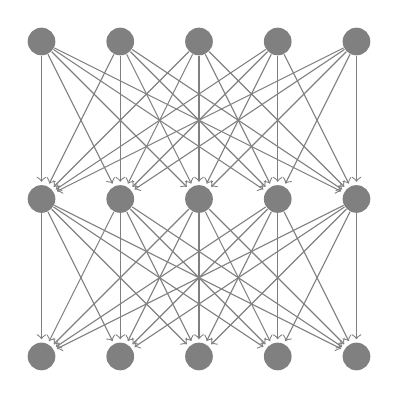
\begin{tikzpicture}[shorten >=1pt,->,draw=black!50, node distance=1cm]
    \tikzstyle{every pin edge}=[<-,shorten <=1pt]
    \tikzstyle{neuron}=[circle,fill=black!50,minimum size=10pt,inner sep=0pt]

    % Draw the hidden layer nodes
    \foreach \name / \x in {1,...,5}
        \path[yshift=0.5cm]
            node[neuron] (I-\name) at (\x,-0cm) {};

    \foreach \name / \x in {1,...,5}
        \path[yshift=0.5cm]
            node[neuron] (H-\name) at (\x,-2cm) {};

    \foreach \source in {1,...,5}
        \foreach \dest in {1,...,5}
            \path (I-\source) edge (H-\dest);

    \foreach \name / \x in {1,...,5}
        \path[yshift=0.5cm]
            node[neuron] (K-\name) at (\x,-4 cm) {};

    \foreach \source in {1,...,5}
        \foreach \dest in {1,...,5}
            \path (H-\source) edge (K-\dest);
\end{tikzpicture}


The base input ofor this network is a (unicode) character, which is one-hot encoded before being fed into the recurrent layers.  For training, the network is unrolled to a length of 256 characters, which is about the length of an average
message in our database.  All strings are padded or truncated to a length of 256 characters.


\begin{minted}{python}
  SEQ_LENGTH = 256
  E_DIM = 128
  STATE_DIM = 512
  NUM_CLASSES = 4
  def inference():
      model_input = tf.placeholder('uint8', shape=[None, SEQ_LENGTH])
      _ = tf.one_hot(Globals.model_input, depth=E_DIM, axis=-1)
      _ = tf.reshape(_, [-1, SEQ_LENGTH, E_DIM])
      fw = multi_layer_rnn(N_LAYERS, STATE_DIM)
      bw = multi_layer_rnn(N_LAYERS, STATE_DIM)
      output, _ = tf.nn.bidirectional_dynamic_rnn(fw, bw, _, dtype=tf.float32)
      fw_output = tf.reshape(output[0][:, -1:], [-1, STATE_DIM])
      bw_output = tf.reshape(output[1][:, :1], [-1, STATE_DIM])
      f = project(fw_output, E_DIM)
      b = project(bw_output, E_DIM)
      e = tf.add(f, b)
      Globals.model_output = project(e, NUM_CLASSES)
      Globals.prediction = tf.cast(tf.argmax(Globals.model_output, 1), tf.uint8)
      return Globals.model_input, Globals.model_output
\end{minted}

first hour:
Loss: 1.331 Accuracy: 45.50%
0	Negative	Neutral	Positive	Irrelevant
Negative	291	113	50	127
Neutral	108	164	62	85
Positive	0	0	0	0
Irrelevant	0	0	0	0


Loss: 0.933 Accuracy: 60.30%
0	Negative	Neutral	Positive	Irrelevant
Negative	292	52	36	55
Neutral	61	176	21	62
Positive	5	15	65	15
Irrelevant	33	28	14	70


second hour
Loss: 0.729 Accuracy: 71.80%
0	Negative	Neutral	Positive	Irrelevant
Negative	340	67	18	65
Neutral	22	182	18	36
Positive	10	7	91	10
Irrelevant	8	13	8	105

third hour
Loss: 0.611 Accuracy: 76.70%
0	Negative	Neutral	Positive	Irrelevant
Negative	319	38	11	43
Neutral	20	188	2	20
Positive	10	18	91	10
Irrelevant	27	27	7	169

Loss: 0.468 Accuracy: 85.20%
0	Negative	Neutral	Positive	Irrelevant
Negative	334	20	3	18
Neutral	14	242	0	9
Positive	20	10	125	17
Irrelevant	26	10	1	151

0	Negative	Neutral	Positive	Irrelevant
Negative	334	4	4	9
Neutral	3	283	2	7
Positive	1	0	125	2
Irrelevant	1	0	4	221

Loss: 0.530 Accuracy: 84.60%
0	Negative	Neutral	Positive	Irrelevant
Negative	361	18	13	29
Neutral	22	246	10	18
Positive	6	6	95	6
Irrelevant	11	5	10	144


Loss: 0.275 Accuracy: 90.00%
0	Negative	Neutral	Positive	Irrelevant
Negative	321	16	3	20
Neutral	8	286	4	6
Positive	4	2	125	16
Irrelevant	11	9	1	168

\subsection{Many-to-many} 

\begin{tikzpicture}[shorten >=1pt,->,draw=black!50, node distance=1cm]
    \tikzstyle{arrow} = [thick,->,>=stealth]
    \tikzstyle{startstop} = [rectangle, minimum width=1.5cm, minimum height=.6cm, text centered, draw=black, fill=black!20]
    \node (input) [] at (0cm,1cm) {};
    \node (output) [] at (0cm,-3cm) {};
    \node (s-input-A) [] at (-2cm,0cm) {};
    \node (s-output-A) [] at (10cm,0cm) {};
    \node (s-input-B) [] at (-2cm,-1cm) {};
    \node (s-output-B) [] at (10cm,-1cm) {};
    \node (s-input-C) [] at (-2cm,-2cm) {};
    \node (s-output-C) [] at (10cm,-2cm) {};
    \path[] node[startstop] (A-0) at (0cm,0cm) {};
    \path[] node[startstop] (B-0) at (0cm,-1cm) {};
    \path[] node[startstop] (C-0) at (0cm,-2cm) {};
    \draw [arrow] (input) -- (A);
    \draw [arrow] (s-input-A) -- (A-0);
    \draw [arrow] (s-input-B) -- (B-0);
    \draw [arrow] (s-input-C) -- (C-0);
    \draw [arrow] (A) -- (B);
    \draw [arrow] (B) -- (C);
    \draw [arrow] (C) -- (output);

     \foreach \i/\j in {1/0,2/1,3/2,4/3}
     {
       \node (input-\i) [] at (2*\i cm,1cm) {};
       \node (output-\i) [] at (2*\i cm,-3cm) {};
       \path[] node[startstop] (A-\i) at (2*\i cm,0cm) {};
       \path[] node[startstop] (B-\i) at (2*\i cm,-1cm) {};
       \path[] node[startstop] (C-\i) at (2*\i cm,-2cm) {};
       \draw [arrow] (A-\i) -- (B-\i);
       \draw [arrow] (B-\i) -- (C-\i);
       \draw [arrow] (input-\i) -- (A-\i);
       \draw [arrow] (A-\j) -- (A-\i);
       \draw [arrow] (B-\j) -- (B-\i);
       \draw [arrow] (C-\j) -- (C-\i);
       \draw [arrow] (C-\i) -- (output-\i);
     }
     \draw [arrow] (A-4) -- (s-output-A);
     \draw [arrow] (B-4) -- (s-output-B);
     \draw [arrow] (C-4) -- (s-output-C);

\end{tikzpicture}

\begin{minted}{python}
  SEQ_LENGTH = 256
  E_DIM = 128
  STATE_DIM = 512
  N_LAYERS = 3

  def inference():
      model_input = tf.placeholder('uint8', shape=[None, SEQ_LENGTH])
      _ = tf.one_hot(Globals.model_input, depth=E_DIM, axis=-1)
      encode = multi_layer_rnn(N_LAYERS, STATE_DIM)
      state_tuple = tuple(tf.unstack(Globals.initial_state, axis=0))
      output, state = tf.nn.dynamic_rnn(encode, _,
                                        dtype=tf.float32,
                                        initial_state=state_tuple)
      output = tf.reshape(output, [-1, STATE_DIM])
      output = project(output, E_DIM)
      out = tf.cast(tf.argmax(output, 1), tf.uint8)
      out = tf.reshape(out, [-1, SEQ_LENGTH])
      Globals.generated_sequence = out
      Globals.generated_characters = tf.nn.softmax(output)
      Globals.model_output = output
      Globals.state = state
\end{minted}

\begin{minted}{python}
def generate_text(length, session=None):
    generated_text = ''
    character = [[ord(' ')]]
    istate = np.zeros([N_LAYERS, 1, STATE_DIM])
    while len(generated_text) < length:
        feed_dict = {Globals.model_input: character,
                     Globals.initial_state: istate}
        next_char, state = session.run([Globals.generated_characters,
                                        Globals.state],
                                       feed_dict=feed_dict)
        next_char = np.asarray(next_char).astype('float64')
        next_char = next_char / next_char.sum()
        op = np.random.multinomial
        next_char_id = op(1, next_char.squeeze(), 1).argmax()
        next_char_id = next_char_id if chr(next_char_id) in \
                          string.printable else ord(" ")
        generated_text += chr(next_char_id)
        character = [[next_char_id]]
        istate = state
    return generated_text
\end{minted}

\subsection{Many-to-one-to-many}

As an example of a recurrent neural network performing a task that ordinary neural network
should not be able to perform, we present a sorting function which uses GRU cells. The architecture
of the network is the reason we call it a many-to-one-to-many network.  One level takes a list
of numbers, and produces a vector which we can see as representing all the numbers in the list,
and a second layer uses this output vector as input, and produces the original list, sorted in
increasing order. The training was done using sequences of natural numbers $n\in\{1,...,32\}$, and each
of the training sequences of length $32$.  After about 6 days of training, the accuracy of the network
stabilized at around 95\%, and it is worth noting that eventhough it took a long time to breach
the 90\% accuracy mark, very early on in the training did the network output increasing sequences.

\begin{tikzpicture}[shorten >=1pt,->,draw=black!50, node distance=1cm]
    \tikzstyle{arrow} = [thick,->,>=stealth]
    \tikzstyle{startstop} = [rectangle, minimum width=1.5cm, minimum height=.6cm, text centered, draw=black, fill=black!20]
    \node (input) [] at (0cm,1cm) {};
    \node (output) [] at (0cm,-3cm) {};
    \node (s-input-A) [] at (-2cm,0cm) {};
    \node (s-output-A) [] at (10cm,0cm) {};
    \node (s-input-B) [] at (-2cm,-1cm) {};
    \node (s-output-B) [] at (10cm,-1cm) {};
    \node (s-input-C) [] at (-2cm,-2cm) {};
    \node (s-output-C) [] at (10cm,-2cm) {};
    \path[] node[startstop] (A-0) at (0cm,0cm) {};
    \path[] node[startstop] (B-0) at (0cm,-1cm) {};
    \path[] node[startstop] (C-0) at (0cm,-2cm) {};
    \draw [arrow] (input) -- (A);
    \draw [arrow] (s-input-A) -- (A-0);
    \draw [arrow] (s-input-B) -- (B-0);
    \draw [arrow] (s-input-C) -- (C-0);
    \draw [arrow] (A) -- (B);
    \draw [arrow] (B) -- (C);
    \draw [arrow] (C) -- (output);

     \foreach \i/\j in {1/0,2/1,3/2,4/3}
     {
       \node (input-\i) [] at (2*\i cm,1cm) {};
       \node (output-\i) [] at (2*\i cm,-3cm) {};
       \path[] node[startstop] (A-\i) at (2*\i cm,0cm) {};
       \path[] node[startstop] (B-\i) at (2*\i cm,-1cm) {};
       \path[] node[startstop] (C-\i) at (2*\i cm,-2cm) {};
       \draw [arrow] (A-\i) -- (B-\i);
       \draw [arrow] (B-\i) -- (C-\i);
       \draw [arrow] (input-\i) -- (A-\i);
       \draw [arrow] (A-\j) -- (A-\i);
       \draw [arrow] (B-\j) -- (B-\i);
       \draw [arrow] (C-\j) -- (C-\i);
       \draw [arrow] (C-\i) -- (output-\i);
     }
     \draw [arrow] (A-4) -- (s-output-A);
     \draw [arrow] (B-4) -- (s-output-B);
     \draw [arrow] (C-4) -- (s-output-C);

\end{tikzpicture}

\begin{minted}{python}
  SEQ_LENGTH = 256
  E_DIM = 128
  STATE_DIM = 512
  N_LAYERS = 4

  def inference():
      model_input = tf.placeholder('uint8', shape=[None, SEQ_LENGTH])
      _ = tf.one_hot(Globals.model_input, depth=E_DIM, axis=-1)
      _ = tf.reshape(_, [-1, SEQ_LENGTH, E_DIM])
      encode = multi_layer_rnn(N_LAYERS, STATE_DIM)
      encoded_input, state = tf.nn.dynamic_rnn(encode,
                                               _,
                                               dtype=tf.float32)
      Globals.encoder_output = state
      with tf.variable_scope('decoder'):
          training_decoder_input = tf.zeros_like(Globals.model_input)
          _ = tf.one_hot(training_decoder_input, depth=E_DIM, axis=-1)
          _ = tf.reshape(_, [-1, SEQ_LENGTH, E_DIM])
          decode = multi_layer_rnn(N_LAYERS, STATE_DIM)
          decoded_output, state = tf.nn.dynamic_rnn(decode, _,
                                                    dtype=tf.float32,
                                                    initial_state=state)
          decoded_output = tf.reshape(decoded_output, [-1, STATE_DIM])
          output = project(decoded_output, E_DIM)
          out = tf.cast(tf.argmax(output, 1), tf.uint8)
          out = tf.reshape(out, [-1, SEQ_LENGTH])
          Globals.training_decoder_input = training_decoder_input
          Globals.model_output = output
          Globals.prediction = out
          Globals.decoder = decode
          Globals.decoder_input = _
\end{minted}


\end{document}
